\section{Phương trình mặt phẳng trong không gian}
\subsection{Đề 1}
\Opensolutionfile{ans}[ans/ans-0-B15]
\caulc
\begin{ex}%[2H5N1-2]
	Trong không gian $Oxyz$, cho mặt phẳng $(P)\colon x-2 y+3 z+1=0$. Hỏi véc-tơ nào dưới đây là một véc-tơ pháp tuyến của mặt phẳng $(P)$?
	\choice
	{\True $(1;-2; 3)$}
	{$(1; 2; 3)$}
	{$(-2; 3; 1)$}
	{$(2;-2; 4)$}
	\loigiai{
		Véc-tơ $(1;-2; 3)$ là một véc-tơ pháp tuyến của mặt phẳng $(P)$.
	}
\end{ex}
\begin{ex}%[2H5N1-4]
	Trong không gian $Oxyz$, cho hai mặt phẳng $(P)\colon x-y-2z+1=0$ và $(Q)\colon mx+(3-2m)y+nz+1=0$. Khi hai mặt phẳng $(P)$ và $(Q)$ song song với nhau thì giá trị của biểu thức $T=m+n$ bằng
	\choice
	{$1$}
	{$0$}
	{\True $-3$}
	{$5$}
	\loigiai{
		Hai mặt phẳng $(P)$ và $(Q)$ song song với nhau khi và chỉ khi \[\dfrac{m}{1}=\dfrac{3-2m}{-1}=\dfrac{n}{-2}\neq \dfrac{1}{1}\Leftrightarrow \heva{&m=3\\&n=-6.}\]
		Vậy $T=m+n=3-6=-3$.
	}
\end{ex}

\begin{ex}%[2H5H1-3]
	Trong không gian với hệ trục tọa độ $Oxyz$, cho mặt phẳng $(P)\colon 2x-y-2z-1=0$. Mặt phẳng $(Q)$ đi qua gốc tọa độ $O$ và song song với $(P)$ là
	\choice
	{$2x+y-2z=0$}
	{\True $2x-y-2z=0$}
	{$2x-y-2z+1=0$}
	{$2x+2y-z=0$}
	\loigiai{
		Mặt phẳng $(Q)$ song song với $(P)$ nên mặt phẳng $(Q)$ có dạng $2x-y-2z+d=0$ ($ d\neq -1 $).\\
		Mặt phẳng $(Q)$ đi qua gốc $O$ nên $ d=0 $ (thỏa mãn).\\
		Vậy $(P)\colon 2x-y-2z=0$. 
	}
\end{ex}


\begin{ex}%[2H5H1-3]
	Trong không gian $Oxyz$, mặt phẳng $(\alpha)$ đi qua điểm $A(1;2;-3)$ và nhận véc-tơ $\overrightarrow{n}=(2;-1;3)$ làm véc-tơ pháp tuyến có phương trình là
	\choice
	{$x+2y-3z+9=0$}
	{$x+2y-3z-9=0$}
	{\True $2x-y+3z+9=0$}
	{$2x-y+3z-9=0$}
	\loigiai{
		Mặt phẳng $(\alpha)$ đi qua điểm $A(1;2;-3)$ và nhận véc-tơ $\overrightarrow{n}=(2;-1;3)$ làm véc-tơ pháp tuyến có phương trình
		$$2(x-1)-(y-2)+3(z+3)=0 \Leftrightarrow 2x-y+3z+9=0.$$
	}
\end{ex}

\begin{ex}%[2H5N1-1]
	Trong không gian $Oxyz$, điểm $M(1;-3;2)$ thuộc mặt phẳng có phương trình nào sau đây?
	\choice 
	{\True$2x+y-z+3=0$}
	{$3x-y+z-2=0$}
	{$2x+y-z+4=0$}
	{$x-2y-z+1=0$}
	\loigiai{ Thay toạ độ điểm $M(1;-3;2)$ lần lượt vào các mặt phẳng ta được
		\begin{itemize}
			\item $3\cdot 1-1\cdot (-3)+1\cdot 2-2\neq 0$. Do đó $M$ không thuộc mặt phẳng $2x+y-z+3=0$.
			\item $2\cdot 1+1\cdot (-3)-1\cdot 2+4\neq 0$. Do đó $M$ không thuộc mặt phẳng $2x+y-z+4=0$.
			\item $1\cdot 1-2\cdot (-3)-1\cdot 2+1\neq 0$. Do đó $M$ không thuộc mặt phẳng $x-2y-z+1=0$.
			\item $2\cdot 1+1\cdot (-3)-1\cdot 2+3=0$. Do đó $M$ thuộc mặt phẳng $2x+y-z+3=0$.
		\end{itemize}
	}
\end{ex}
\begin{ex}%[2H5H1-3]
	Trong không gian $Oxyz$, cho hai điểm $A(-1;2;0)$, $B(1;1;3)$ và mặt phẳng $(P)\colon x-2y+3z-5=0$. Phương trình của mặt phẳng đi qua hai điểm $A$, $B$ đồng thời vuông góc với $(P)$ là
	\choice
	{$x+2y+z-3=0$}
	{$2x+y-z=0$}
	{\True $x-y-z+3=0$}
	{$x+y-z-1=0$}
	\loigiai
	{
		Ta có $\overrightarrow{AB}=(2;-1;3)$ và véc-tơ pháp tuyến của mặt phẳng $(P)$ là $\overrightarrow{n}_P=(1;-2;3)$.\\
		Gọi $(Q)$ là mặt phẳng đi qua $A$, $B$ và vuông góc $(P)$.\\
		Khi đó véc-tơ pháp tuyến của mặt phẳng $(Q)$ là $$\overrightarrow{n}_Q=\left[\overrightarrow{AB}, \overrightarrow{n}_P\right]=(3;-3;-3)=3(1;-1;-1).$$
		Vậy phương trình mặt phẳng $(Q)$ đi qua $A(-1;2;0)$ và có véc-tơ pháp tuyến $\overrightarrow{n}_Q=(1;-1;-1)$ có phương trình
		$$(Q)\colon x-y-z+3=0.$$
	}
\end{ex}


\begin{ex}%[2H5N1-1]
	Trong không gian $Oxyz$, mặt phẳng $(P)\colon x+2y-2z+1=0$ đi qua điểm nào dưới đây?
	\choice
	{\True $M(1;2;3)$}
	{$N(1;2;-2)$}
	{$P(-1;2;-3)$}
	{$Q(2;-2;1)$}
	\loigiai{
		Thay tọa độ các điểm $M$, $N$, $P$, $Q$ vào phương trình mặt phẳng $(P)$ ta thấy chỉ có điểm $M$ có tọa độ thỏa mãn.\\
		Vậy		mặt phẳng $(P)\colon x+2y-2z+1=0$ đi qua điểm $M(1;2;3)$.
	}
\end{ex}	

\begin{ex}%[2H5H1-3]
	Trong không gian $Oxyz$, cho hai điểm $A(-1;0;2)$, $B(3;2;0)$. Phương trình mặt phẳng trung trực của $AB$ là
	\choice
	{$x+y+z+2=0$}
	{$2 x+y-z+2=0$}
	{$x+y+z-2=0$}
	{\True $2x+y-z-2=0$}
	\loigiai{
		Ta có $\overrightarrow{AB}=(4;2;-2)$.\\
		Gọi $(P)$ là mặt phẳng trung trực của $AB$. Ta có phương trình $(P)$ đi qua trung điểm $I(1;1;1)$ của $AB$ và nhận $\overrightarrow{n}=(2;1;-1) $ làm một véc-tơ pháp tuyến là
		\[ 2(x-1)+(y-1)-(z-1)=0\Leftrightarrow 2x+y-z-2=0.\]
	}
\end{ex}
\begin{ex}%[2H5H1-3]
	Trong không gian với hệ trục tọa độ $Oxyz$, cho điểm $M(1;2;3)$. Gọi $A$, $B$, $C$ lần lượt là hình chiếu vuông góc của điểm $M$ lên các trục $Ox$, $Oy$, $Oz$. Phương trình mặt phẳng $(ABC)$ là
	\choice
	{\True $\dfrac{x}{1}+\dfrac{y}{2}+\dfrac{z}{3}=1$}
	{$-\dfrac{x}{1}+\dfrac{y}{2}+\dfrac{z}{3}=1$}
	{$\dfrac{x}{1}+\dfrac{y}{2}+\dfrac{z}{3}=0$}
	{$\dfrac{x}{1}-\dfrac{y}{2}+\dfrac{z}{3}=1$}
	\loigiai{
		Ta có điểm $M(1;2;3)$ có hình chiếu vuông góc lên các trục $Ox$, $Oy$, $Oz$ là $A(1;0;0)$, $B(0;2;0)$, $C(0;0;3)$.\\
		Do đó phương trình mặt phẳng $(ABC)\colon \dfrac{x}{1}+\dfrac{y}{2}+\dfrac{z}{3}=1$.
	}
\end{ex}






\begin{ex}%[2H5N1-5]
	Trong không gian $Oxyz$, cho điểm $M(-1;2;0)$ và mặt phẳng $(P)\colon 2x-2y+z+1=0$. Tính khoảng cách từ điểm $M$ đến mặt phẳng $(P)$.
	\choice
	{$-\dfrac{5}{3}$}
	{$\dfrac{7}{3}$}
	{\True $\dfrac{5}{3}$}
	{$ 5 $}
	\loigiai{
		Khoảng cách từ điểm $ M $ đến $ (P) $ là
		$$ \mathrm{d}(M,(P))=\dfrac{|2\cdot (-1)-2\cdot 2+0+1|}{\sqrt{2^2+(-2)^2+1^2}}=\dfrac{|-5|}{\sqrt{9}}=\dfrac{5}{3}.$$}
\end{ex}


\begin{ex}%[2H5H1-3]
	Phương trình mặt phẳng $(P)$ chứa hai điểm $A(2;1;1)$; $B(3;-2;4)$ và song song với $CD$, $C(-2;3;1)$; $D(-3;4;-6)$ có dạng $(P)\colon 9x + by + cx + d = 0$. Giá trị của $b + c + d$ bằng
	\choice 
	{$-19$}
	{\True $-18$}
	{$-17$}
	{$-20$}
	\loigiai{
		Ta có $\overrightarrow{AB} = (1;-3;3)$, $\overrightarrow{CD} = (-1;1;-7)$.\\
		Vì mặt phẳng $(P)$ chứa hai điểm $A(2;1;1)$; $B(3;-2;4)$ và song song với $CD$ nên $(P)$ nhận $\overrightarrow{n} = \left[ \overrightarrow{AB};\overrightarrow{CD} \right] = (18;4;-2)$ làm một véc-tơ pháp tuyến.\\
		Mặt phẳng $(P)$ đi qua điểm $A(2;1;1)$ và có véc-tơ pháp tuyến $\overrightarrow{n'} = (9;2;-1)$ nên có phương trình là
		$$ 9(x-2) + 2(y-1) - 1(z-1) = 0 \Leftrightarrow 9x + 2y - z - 19 = 0. $$
		Vậy $b = 2$, $c = -1$, $d = -19$ do đó $b + c + d = 2 + (-1) + (-19) = -18$.
	}
\end{ex}

\begin{ex}%[2H5H1-3]
	Mặt phẳng $(P)$ đi qua điểm $A(2;3;-5)$ và chứa trục $Ox$ có phương trình là
	\choice 
	{$y = 0$}
	{$3y - 5z = 0$}
	{\True $5y + 3z = 0$}
	{$y - z = 0$}
	\loigiai{
		Trục $Ox$ đi qua $O(0;0;0)$ và có $\overrightarrow{i} = (1;0;0)$, $\overrightarrow{OA} = (2;3;-5)$.\\
		Ta có $\overrightarrow{n} = \left[ \overrightarrow{OA};\overrightarrow{i} \right] = (0;-5;-3)$.\\
		Mặt phẳng $(P)$ đi qua điểm $A(2;3;-5)$ và nhận $\overrightarrow{n} = (0;-5;-3)$ làm một véc-tơ pháp tuyến có phương trình là
		$$ 0(x-2) - 5(y - 3) - 3(z + 5) = 0 \Leftrightarrow -5y - 3z = 0 \Leftrightarrow 5y + 3z = 0. $$
	}
\end{ex}

\Closesolutionfile{ans}
\indapan{6}{ans/ans-0-B15}

\cauds
\Opensolutionfile{ans}[ans/ans-0-B15-DS]

\begin{ex}%[2H5N1-2]
	Trong không gian $Oxyz$, cho mặt phẳng $(P)\colon x-3y+2z-3=0$. Các khẳng định sau là đúng hay sai?
	\choiceTF
	{\True $\vec{n_1}=(1;-3;2)$ là một véc-tơ pháp tuyến của $(P)$}
	{\True $\vec{n_2}=(-4;12;-8)$ là một véc-tơ pháp tuyến của $(P)$}
	{\True $\vec{n_3}=(-2;6;-4)$ không phải là một véc-tơ pháp tuyến của $(P)$}
	{$\vec{n_4}=(1;-2;3)$ là một véc-tơ pháp tuyến của $(P)$}
	\loigiai{
		Mặt phẳng $(P)$ có một véc-tơ pháp tuyến là $\vec{n_1}=(1;-3;2)$, nên $(P)$ có hai véc-tơ pháp tuyến khác là $\vec{n_2}=(-4;12;-8)$ và $\vec{n_3}=(-2;6;-4)$. Véc-tơ $\vec{n_4}=(1;-2;3)$ không phải là một véc-tơ pháp tuyến của $(P)$. 
	}
\end{ex}
\begin{ex}%[2H5H1-2]
	Trong không gian $Oxyz$, cho mặt phẳng $(P)$ đi qua ba điểm $A(1;0;2)$, $B(-1;2;1)$, $C(2;-3;1)$. Các khẳng định sau là đúng hay sai?
	\choiceTF
	{\True Mặt phẳng $(P)$ có một cặp véc-tơ chỉ phương là $\vec{u_1}=(-2;2;-1)$ và $\vec{u_2}=(3;-5;0)$}
	{\True Mặt phẳng $(P)$ có một véc-tơ pháp tuyến là $\vec{n}=(-5;-3;4)$}
	{Mặt phẳng $(P)$ có một véc-tơ pháp tuyến là $\vec{n}=(5;3;4)$}
	{\True Mặt phẳng $(P)$ có một véc-tơ pháp tuyến là $\vec{n}=(10;6;-8)$}
	\loigiai{
		Mặt phẳng $(P)$ đi qua ba điểm $A(1;0;2)$, $B(-1;2;1)$, $C(2;-3;1)$ nên $(P)$ nhận $\break \vec{AB}=(-2;2;-1)$ và $\vec{BC}=(3;-5;0)$ làm cặp véc-tơ chỉ phương. \\
		Do đó, ta có thể chọn véc-tơ $\vec{n}=[\vec{AB},\vec{BC}]=(-5;-3;4)$ làm một véc-tơ pháp tuyến của $(P)$.\\
		Vậy véc-tơ $(10;6;-8)$ cũng là một véc-tơ pháp tuyến của $(P)$.
	}
\end{ex}


\begin{ex}%[2H5H1-4]
	Trong không gian $Oxyz$, cho hai mặt phẳng $(P)\colon 2x-y+3z+1=0$ và $(Q)\colon -4x+by+cz+5=0$. Các khẳng định sau là đúng hay sai?
	\choiceTF
	{\True $(P)\parallel (Q)\Leftrightarrow b=2, c=-6$}
	{Tồn tại giá trị của $b$ và $c$ để $(P)\equiv (Q)$}
	{\True Với $b=1$ và $c=2$ thì $(P)$ cắt $(Q)$}
	{\True Với $b=1$ và $c=3$ thì $(P)\perp (Q)$}
	\loigiai{
		\begin{itemchoice}
			\itemch Ta có $(P)\parallel (Q)\Leftrightarrow \dfrac{2}{-4}=\dfrac{-1}{b}=\dfrac{3}{c}\neq \dfrac{1}{5}\Leftrightarrow b=2, c=-6$.
			\itemch Ta có $(P)\equiv (Q)\Leftrightarrow \dfrac{2}{-4}=\dfrac{-1}{b}=\dfrac{3}{c}= \dfrac{1}{5}$. Hệ phương trình này vô nghiệm vì $\dfrac{2}{-4}\neq \dfrac{1}{5}$ nên không tồn tại giá trị của $b$ và $c$ để hai mặt phẳng trùng nhau.
			\itemch Với $b=1$ và $c=2$ ta có $\dfrac{2}{-4}\neq \dfrac{-1}{1}\neq \dfrac{3}{2}$ nên hai mặt phẳng $(P)$ và $(Q)$ cắt nhau.
			\itemch Với $b=1$ và $c=3$, ta có $\vec{n}_{(P)}=(2;-1;3)$ và $\vec{n}_{(Q)}=(-4;1;3)$. Ta có $\vec{n}_{(P)}\cdot \vec{n}_{(Q)}=-8-1+9=0$. Do đó $(P)\perp (Q)$.
		\end{itemchoice}
	}
\end{ex}
\begin{ex}%[2H5H1-6]
	Trong không gian với hệ tọa độ $Oxyz$ cho hai mặt phẳng $(P_1)$ và $(P_2)$ có các véc tơ pháp tuyến lần lượt là $\overrightarrow{n_1}$, $\overrightarrow{n_2}$. Gọi $\alpha$ là góc giữa $(P_1)$ và $(P_2)$. Xác định tính đúng, sai của các mệnh đề sau:
	\choiceTF
	{$\alpha=(\overrightarrow{n_1}; \overrightarrow{n_2})$}
	{$\alpha + (\overrightarrow{n_1}; \overrightarrow{n_2}) = 180^\circ$}
	{$\cos\alpha = \cos (\overrightarrow{n_1}; \overrightarrow{n_2})$}
	{\True $\cos\alpha = \left|\cos (\overrightarrow{n_1}; \overrightarrow{n_2})\right|$}
	\loigiai{
		Theo định nghĩa, góc giữa hai mặt phẳng là góc giữa hai đường thẳng lần lượt vuông góc với hai mặt phẳng đó. Như vậy nếu gọi $\alpha$ là góc giữa $(P_1)$ và $(P_2)$ thì $0^\circ \le \alpha \le 90^\circ$.\\
		Trong khi đó: $0^\circ \le (\overrightarrow{n_1}; \overrightarrow{n_2}) \le 180^\circ$.\\
		Như vậy $\heva{& \alpha = (\overrightarrow{n_1}; \overrightarrow{n_2}) & \text{nếu\;} 0^\circ\le (\overrightarrow{n_1}; \overrightarrow{n_2}) \le 90^\circ \\& \alpha = 180^\circ-(\overrightarrow{n_1}; \overrightarrow{n_2}) & \text{nếu\;} (\overrightarrow{n_1}; \overrightarrow{n_2}) > 90^\circ.}$\\
		
	}
\end{ex}





\Closesolutionfile{ans}
\indapan{3}{ans/ans-0-B15-DS}

\Opensolutionfile{ans}[ans/ans-0-B15-KQ]
\caukq

\begin{ex}%[2H5H1-5]
	Trong không gian $Oxyz$, cho $(P)\colon x - y + z - 3 = 0$ và $A(5;6;7)$. Gọi $H(a;b;c)$ là hình chiếu vuông góc của $A$ trên $(P)$. Tính $a + 2b + c$.
	\shortans{$24$}
	\loigiai{
		Mặt phẳng $(P)\colon x - y + z - 3 = 0$ có véc-tơ pháp tuyến $\overrightarrow{n}_{P} = (1;-1;1)$.\\
		Gọi $d$ là đường thẳng đi qua $A(5;6;7)$ và vuông góc với $(P)$. Khi đó đường thẳng $d$ nhận $\overrightarrow{n}_{P} = (1;-1;1)$ làm một véc-tơ chỉ phương nên $d$ có phương trình 
		$$ d\colon \heva{&x = 5 + t\\&y = 6 - t\\&z = 7 + t.} $$
		Vì $H(a;b;c)$ là hình chiếu vuông góc của $A$ trên $(P)$ nên $H \in d \Rightarrow H(5+t;6-t;7+t)$ và $H \in (P)$ do đó
		$$ (5+t) - (6-t) + (7+t) - 3 = 0 \Leftrightarrow t = -1. $$
		Suy ra $H(4;7;6)$, do đó $a + 2b + c = 4 + 2\cdot 7 + 6 = 24$.
	}
\end{ex}

\begin{ex}%[2H5V1-6]
	Trong không gian với hệ tọa độ $Oxyz$, cho các điểm $A(1;0;0)$, $B(0;2;0)$, $C(0;0;m)$. Để mặt phẳng $(ABC)$ hợp với mặt phẳng $(Oxy)$ một góc $60^\circ$ thì tổng các giá trị của $m$ là
	\shortans{$0$}
	\loigiai{
		Mặt phẳng $Oxy$ có véc-tơ pháp tuyến là $\overrightarrow{k}=(0;0;1)$.\\
		Ta có $\overrightarrow{AB}=(-1;2;0)$ và $\overrightarrow{AC}=(-1;0;m)$, suy ra véc-tơ pháp tuyến của mặt phẳng $(ABC)$ là $\overrightarrow{n}=\left[\overrightarrow{AB},\overrightarrow{AC}\right]=(2m;m;2)$.\\
		Theo bài ra ta có
		$$\cos60^\circ=\dfrac{\left|\overrightarrow{k}\cdot\overrightarrow{n}\right|}{|\overrightarrow{k}|\cdot|\overrightarrow{n}|}$$
		$$\Leftrightarrow \sqrt{5m^2+4}=4\Leftrightarrow m^2=\dfrac{12}{5}\Leftrightarrow m=\pm\sqrt{\dfrac{12}{5}}.$$
		Vậy tổng các giá trị $m$ thỏa bài toán là $0$.
	}
\end{ex}

\begin{ex}%[2H5V1-5]
	Trong không gian cho hai điểm $ A(2;-2;2) $, $ B(4;2;-1) $ và mặt phẳng $ (P)\colon (m+2n)x+(m-1)y +(n+2)z-6=0$. Gọi $ H $ là hình chiếu vuông góc của $ A $ lên mặt phẳng $ (P) $. Khi hai tham số $ m $, $ n $ thay đổi, quỹ tích điểm $ H $ luôn cách $ B $ một đoạn bằng $ \sqrt{21} $ là đường tròn có bán kính bằng bao nhiêu (làm tròn đến hàng phần trăm)?
	\shortans{$2{,}24$}
	\loigiai{Giả sử $ C(x_0,y_0,z_0) $ là điểm cố định thuộc $ (P) $ khi $ m,n $ thay đổi, tức là
		$$\begin{array}{lll}
			&&(m+2n)x_0+(m-1)y_0 +(n+2)z_0-6=0\\
			& \Leftrightarrow & m\left(x_0+y_0\right)+n\left(2x_0+z_0\right)-y_0+2z_0-6=0,\,\forall m,n\in\mathbb{R}\\
			&\Leftrightarrow&\heva{&x_0+y_0=0\\&2x_0+z_0=0\\&-y_0+2z_0-6=0}\\\
			&\Rightarrow& C(-2;2;4).
		\end{array} $$
		\immini{Do $ \widehat{AHC}=90^\circ$ nên $ H \in (C)$ là mặt cầu đường kính $ (AC) $, có tâm $ I(0;0;3) $ và bán kính $ R= 3$.\\
			Do $ HB = \sqrt{21}$ nên $ H $ thuộc mặt cầu tâm $ B(4;2;-1) $, bán kính $ R'=HB=\sqrt{21} $.\\
			Khi đó quỹ tích $H$ là đường tròn giao tuyến của hai mặt cầu tâm $ I(0;0;3) $ và bán kính $ R= 3$ và mặt cầu tâm $ B(4;2;-1) $, bán kính $ R'=HB=\sqrt{21} $.\\
			Gọi $ r $ là bán kính đường tròn quỹ tích của $ H $, ta có 
			$$ \sqrt{9-r^2} +\sqrt{21-r^2}=IB=6\Leftrightarrow r=\sqrt{5}.$$}{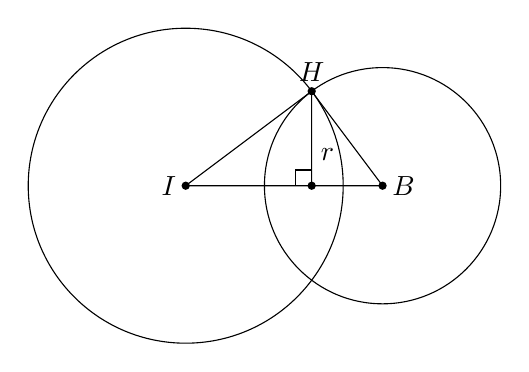
\begin{tikzpicture}[>=stealth,x=1cm,y=1cm,scale=1]
				\fill[black] (-1,0)node[left]{\normalsize $I$} circle (1.5pt);
				\fill[black] (1.5,0)node[right]{\normalsize $B$} circle (1.5pt);
				\fill[black] (0.6,1.2)node[above]{\normalsize $H$} circle (1.5pt);
				\fill[black] (0.6,0) circle (1.5pt);
				\draw(-1,0) circle (2cm);
				\draw(1.5,0) circle (1.5cm);
				\draw (-1,0)--(0.6,1.2)--(1.5,0)--cycle (0.6,0)--(0.6,1.2);
				\node at (0.8,0.4) {$ r $};
				\draw (0.6,0)--(0.6,0.2)--(0.4,0.2)--(0.4,0);
		\end{tikzpicture}}
	}
\end{ex}


\begin{ex}%[2H5V1-5]
	Trong không gian $Oxyz$, cho hai điểm $A(1;-1;3)$, $B(3;2;2)$. Biết rằng hai điểm $A$ và $B$ nằm khác phía so với mặt phẳng $ (\alpha)\colon ax+by+3z+d=0 $, với $ a $ và $ d $ là những tham số. Biết rằng tổng khoảng cách từ $ A $ và $ B $ đến $ (\alpha) $ lớn nhất. Giá trị nguyên dương lớn nhất của $ d $ là
	\shortans{$29$}
	\loigiai{
		\immini
		{Vì $ A $, $ B $ khác phía đối với $ (\alpha) $ nên gọi $I$ là giao điểm của đoạn thẳng $AB $ và $ (\alpha) $, gọi $ H $, $ K $ lần lượt là hình chiếu vuông góc của $ A $ và $ B $ trên mặt phẳng $ (\alpha) $, ta có 
			\begin{eqnarray*}
				T&=&\mathrm{d}\left(A,(\alpha)\right)+\mathrm{d}\left(B,(\alpha)\right)\\
				&=&AH+BK\\
				&\le & AI+ BI=AB.
			\end{eqnarray*}
			Dấu \lq\lq$=$\rq\rq\, xảy ra khi và chỉ khi $\heva{&\mathrm{d}\left(A,(\alpha)\right)=AI \\ & \mathrm{d}\left(B,(\alpha)\right)=BI} \Leftrightarrow AB \perp \left(\alpha\right)$.}
		{\begin{tikzpicture}[line join=round, line cap=round,scale=0.8]
				\path
				(2,2) coordinate (M)
				(9,2) coordinate (N)
				(0,0) coordinate (Q)
				($(N)+(Q)-(M)$) coordinate (P)
				(4,1) coordinate (I)
				(3,1) coordinate (H)
				(6,1) coordinate (K)
				(3,3) coordinate (A)
				(6,-3) coordinate (B)
				;
				\path[name path=ah] (A)--(H);
				%				\path[name path=ah] (A)--(H)--([turn]0:5cm);
				\path[name path=ab] (A)--(B);
				\path[name path=mn] (M)--(N);
				\path[name path=pq] (P)--(Q);
				\path[name path=bk] (B)--(K);
				\path[name intersections={of=ah and mn,by=E}];
				\path[name intersections={of=ab and mn,by=F}];
				\path[name intersections={of=ab and pq,by=G}];
				\path[name intersections={of=bk and pq,by=J}];
				\draw
				
				(M)--(E) (F)--(N)--(P)--(Q)--(M)
				(A)--(I)--(H)--cycle (G)--(B)--(J) (I)--(K)
				;
				\draw[dashed]
				(E)--(F) (I)--(G) (K)--(J)
				;
				\foreach \i/\g in {A/90,B/-90,I/60,H/180,K/0}
				{\draw[fill=black](\i) circle (1pt) ($(\i)+(\g:3mm)$) node[scale=1]{$\i$};}
				\draw pic[draw,,angle radius=9mm]{angle=P--Q--M};
				\draw pic["$\alpha$",-stealth,angle radius=9mm]{angle=P--Q--M};
		\end{tikzpicture}}
		\noindent
		Suy ra $T$ lớn nhất khi $ \left(\alpha\right) \perp AB$ hay $ \vec{AB}=(2;3;-1) $ là một véc-tơ pháp tuyến của $ (\alpha)$.\\
		Ta có $\vec{AB}$ cùng phương với $\vec{n}=(a;b;3)$ khi và chỉ khi
		\[\dfrac{a}{2}=\dfrac{b}{3}=\dfrac{3}{-1} \Rightarrow \heva{& a=-6 \\ & b=-9.}\]
		Phương trình $ (\alpha)\colon-6x-9y+3z+d=0$.\\
		Vì $ A $, $ B $ khác phía đối với $ (\alpha) $ nên 
		\[(-6+9+9+d)\cdot(-18-18+6+d)<0\Leftrightarrow-12<d<30.\]
		Vậy số nguyên $ d $ lớn nhất bằng $ 29$.
	}
\end{ex}



\begin{ex}%[2H5V1-3]
	Trong không gian $Oxyz$, cho hai điểm $A(2;4;1)$, $B(-1;1;3)$ và mặt phẳng $(P)\colon x-3y+2z-5=0$. Mặt phẳng $(Q)$ đi qua $A$, $B$ và vuông góc với $(P)$ có phương trình dạng $ax+by+cz+11=0$. Tổng $a+b+c$ bằng
	\shortans{$-5$}
	\loigiai
	{Ta có $\overrightarrow{AB}=(-3;-3;2)$, véc-tơ $\overrightarrow{n}=(1;-3;2)$ là véc-tơ pháp tuyến của $(P)$.\\
		Mặt phẳng $(Q)$ đi qua hai điểm $A$, $B$ và vuông góc với mặt phẳng $(P)$ nên nhận véc-tơ $\left[\overrightarrow{AB}, \overrightarrow{n}\right] = (0;8;12)$ làm véc-tơ pháp tuyến. Do đó phương trình $(Q)$ là
		$$8(y-4)+12(z-1)=0 \Leftrightarrow 2y+3z-11=0 \Leftrightarrow -2y-3z+11=0.$$
		Vậy $a=0$, $b=-2$, $c=-3$ và $a+b+c=-5$.}
\end{ex}


\begin{ex}%[2H5C1-7]
	Trong không gian $Oxyz$, cho hai điểm $A(2;1;0)$, $B(1;2;0)$ và điểm $M$ di động trên tia $Oz$. Gọi $H$, $K$ lần lượt là hình chiếu vuông góc của $A$ lên $OB$ và $MB$. Đường thẳng $HK$ cắt trục $Oz$ tại điểm $N$. Khi thể tích khối tứ diện $ABMN$ nhỏ nhất thì mặt phẳng $(AHK)$ có dạng $ax+by+cz-4=0$. Giá trị của $a+b+c$ bằng
	\shortans{$1$}
	\loigiai{
		\immini
		{Ta có $A(2;1;0)$, $B(1;2;0)$ $\Rightarrow A,~ B \in (Oxy)$.\\
			Có $\heva{&AK\perp MB\\&AH\perp OB;~AH\perp OM \Rightarrow AH \perp (OBM) \Rightarrow AH \perp MB}$ mà $AK\perp MB$ nên 
			$ MB \perp (AHK)$.\\
			Gọi $M(0;0;m)$, $(m>0)$ thuộc tia $Oz$ khi đó $\overrightarrow{MB}=(1;2;-m)$\\
			$\Rightarrow (AHK)\colon 1(x-2)+2(y-1)-mz=0$.\\
			$\Rightarrow N=HK \cap Oz =(AHK) \cap Oz \Rightarrow N\left(0;0;-\dfrac{4}{m}\right)$.\\
			Ta có
			\allowdisplaybreaks
			$\begin{aligned}[t]
				V_{ABMN}&=V_{M.OAB}+V_{N.OAB}=\dfrac{1}{3}S_{OAB}\cdot OM +\dfrac{1}{3}S_{OAB}\cdot ON\\
				&=\dfrac{1}{3}S_{OAB}(OM+ON)=\dfrac{1}{3}S_{OAB}\cdot MN
			\end{aligned}$\\
			Vì $S_{OAB}$ không đổi nên $V_{ABMN}$ nhỏ nhất khi và chỉ khi $MN$ nhỏ nhất.\\
			Ta có $MN=m+\dfrac{4}{m}\geq 2\sqrt{m\cdot \dfrac{4}{m}}=4$.\\
			Dấu bằng xảy ra khi $m=\dfrac{4}{m}\Rightarrow m=2$.\\
			Vậy $(AHK)\colon x+2y-2z-4=0 \Rightarrow a+b+c=1+2-2=1$.}
		{\begin{tikzpicture}[scale=0.7, font=\footnotesize, line join=round, line cap=round,>=stealth]
				\def\xmin{-2};\def\ymin{-3};\def\xmax{6};\def\ymax{5};
				\coordinate (O) at (0,0);
				\coordinate (B) at (2,-1);
				\coordinate (A) at (3,0);
				\coordinate (M) at (0,2);
				\coordinate (K) at ($(M)+2/5*(B)-2/5*(M)$);
				\coordinate (H) at ($(O)+1/4*(B)-1/4*(O)$);
				\coordinate (N) at (intersection of M--O and K--H);
				\draw (A)--(B)--(O)--(M)--cycle (M)--(B)--(N) (A)--(K)--(N)--(O);
				\draw [dashed] (O)--(A)--(H) (A)--(N);
				\draw[black] pic[draw, angle radius=2mm, angle eccentricity=1.5]{right angle=B--K--A};
				\draw[black] pic[draw, angle radius=2mm, angle eccentricity=1.5]{right angle=B--H--A};
				\foreach \t/\g in {O/180,B/-90,A/0,M/70,K/90,H/200,N/-90}{\draw[fill=white] (\t) circle (1pt) node[shift={(\g:7pt)},font=\scriptsize]{$\t$};}
		\end{tikzpicture}}
	}
\end{ex}


\Closesolutionfile{ans}
\indapan{6}{ans/ans-0-B15-KQ}